% 来源：OEBPS/Text/Section0001_split_008.xhtml#sigil_toc_id_56

\BookChapter{43}
\section[第43章\q 约翰·邓普顿爵士：20世纪最伟大的投资人]{第43章\\ 约翰·邓普顿爵士：20世纪最伟大的投资人}

\begin{figure}[htbp]
\centering
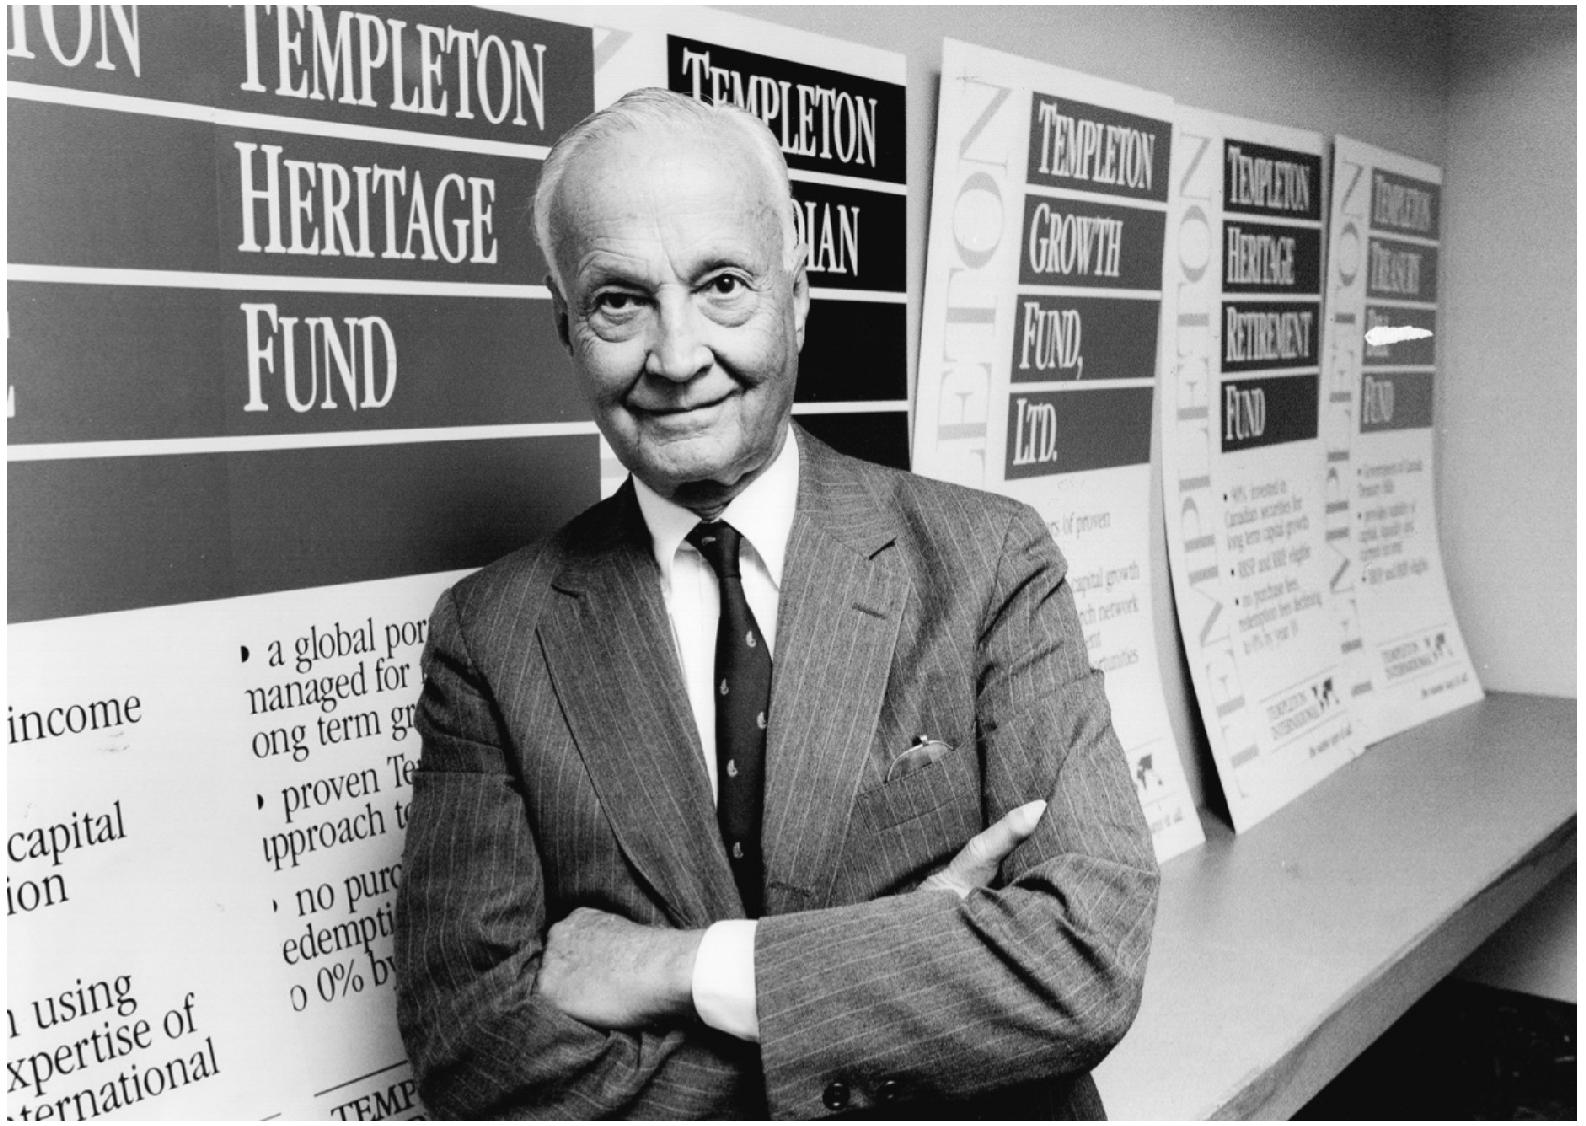
\includegraphics[width=0.54\linewidth,keepaspectratio]{image/约翰·邓普顿爵士肖像.jpg}
\caption*{约翰·邓普顿爵士}
\end{figure}

邓普顿基金公司创始人，慈善家，百万英镑邓普顿奖创立人

约翰·邓普顿爵士，不仅是有史以来最伟大的投资管理大师之一，也是有史以来最伟大的人之一。我很荣幸能够称他为我的导师。邓普顿的信条是“所知愈少而所学愈饥”，这一信条指导了他漫长又光辉灿烂的一生，让他成为一个投资先锋，一个打破传统习俗束缚的人，一个追求精神境界的灵魂，一个慈善家。约翰·邓普顿爵士最为人称道的是，他能够洞察世界上最困难的情况，然后找到办法加以利用，从而获利。

约翰·邓普顿受封“约翰爵士”，不是因为有背景，也不是因为父母有钱，而是靠自己多年奋斗才实现受人尊敬的。他出身很卑微，1912年出生在田纳西州的一个小镇上，家境贫寒，从小到大培养出非常有用的人生价值观：节俭、自立、自律。他非常努力，靠奖学金先上了耶鲁大学，又到牛津大学读了研究生。1937年在华尔街找到了第一份工作，那个时候正是美国经济大萧条最严重的时候。邓普顿天生就是一个逆向投资者，他相信，买股票就要在“市场最悲观的时候”。其他人都觉得世界末日就要来了，邓普顿却认为这正好是投资买入的好时候。其他人都认为：“我的天哪，这是历史上最好的投资时机！”邓普顿却认为这时候应该卖出股票。

邓普顿第一次把他的理论用实践来检验是在1939年秋天，当时美国经济大萧条，希特勒的部队已经开进波兰，“二战”刚刚开始，市场极度恐慌，股市暴跌。邓普顿决定，把他手上存的所有钱都拿出来，又另外借了些钱，纽约交易所里的股票，只要股价是1美元或者低于1美元的，他就每只买上100美元。正是这个熊市里的一美元股组合，成为他个人巨大财富的根基，也成为他资产管理帝国的根基。邓普顿也是国际投资的先锋，其他美国人拒绝跨出美国国境一步的时候，邓普顿已经在全世界到处发掘投资机会了。

财富增长得越多，邓普顿回馈社会的也就越多。1972年，邓普顿建立了世界上奖金最高的年度大奖，颁发给个人的奖金比诺贝尔奖的奖金还要高，用来奖励那些获得巨大精神成就的人士。特蕾沙修女是第一个邓普顿奖获奖人。邓普顿基金会也赞助科技研究。1987年，英国女王伊丽莎白册封邓普顿为爵士，以表彰他对人类做出的巨大贡献。

邓普顿不断演讲和写作，激发了数百万人，他的言语非常谦逊，传达的信息却非常宝贵，主要是关于正直、企业家精神、信仰，一直持续到他2008年去世，享年95岁。（巧合的是，他准确地预测了那一年房地产市场泡沫的破裂。）就在他去世几个月前，我对约翰·邓普顿爵士做了一次访谈，下面就是这次访谈的内容节选。邓普顿和善的光芒闪耀在每个回答上，他分享了自己的哲学，能让你成为伟大投资人的特质，同样也能让你成为一个伟大的人。

\begin{BookQuote}
\textbf{罗宾斯：}约翰·邓普顿爵士，很多人做事，要么是为了钱，要么是为了精神信仰，但是你找到了一条路合二为一，在你的生活中把二者融合在一起，非常自然，又非常紧密。你觉得一般人在生活中能把二者融合到一起吗？
\end{BookQuote}

\begin{BookQuote}
\textbf{邓普顿：}绝对可以！其实二者没有什么差异，你会跟一个你不信任的商人打交道吗？肯定不会！如果有个人名声坏，不值得信任，大家都会躲他远远的，他的企业肯定会失败。如果一个人有很高的道德准则，很高的精神准则，他会努力给他的客户和他的员工贡献更多，比他们预期的还要多，做到这些的人就会很受大家欢迎。他会有更多的客户，赚更多的钱，对这个世界做出更多的贡献，这样自然也会让自己兴旺发达，会有更多的朋友，会更受人尊敬。
\end{BookQuote}

所以，你从一开始要努力给予别人更多，比别人预期会从你这里得到的还要多，对待别人不只是公平，而且是更加优厚，这就是成功的秘诀。不要想占别人的便宜，也不要阻挡别人的进步。你帮助别人越多，你自己就会越兴旺发达。给予的越多，得到的越多。

\begin{BookQuote}
\textbf{罗宾斯：}你的第一笔投资是什么？是什么吸引你做这笔投资的？后来这笔投资的结果怎么样？
\end{BookQuote}

\begin{BookQuote}
\textbf{邓普顿：}我第一次开始投资的时候，正好赶上“二战”刚开战，那是1939年9月。我们刚刚结束了世界上最大的经济大萧条，有很多公司都破产了。但是战争一来，每一种产品的需求都大大增加，结果战争期间，几乎每家公司的生意都重新兴旺发达，所以我非常看好股市，于是我向券商下了单，只要是一元股，就是股票交易价格是1美元，或者更低，就每只买上100美元，当时股市一共有104只这种一元股，我一共买入10400美元。结果后来这104只一元股里有100只股票我都赚钱了，只有4只股票亏损。
\end{BookQuote}

三年之后，我和我太太有机会收购一家规模很小的退休投资顾问公司，我们手上的积蓄正好够收购这家公司！一开始，一个客户都没有。我们公司的办公室就设在纽约的无线电城，我们在那里一直干了25年，我们一直是赚到1美元就存起来50美分，好让我们能够积攒起一些资产，支撑我们以后的退休生活，也支撑我们做慈善活动。

\begin{BookQuote}
\textbf{罗宾斯：}哇！你每赚到1美元，就存起来50美分，我的天哪！你的收入储蓄比例有50\%，这也太高了，我的约翰·邓普顿爵士！大多数人现在都会说“这根本不可能！我不可能从我的收入里拿出一半存起来，然后去投资”。但是，正是靠着平时把一半收入存起来，你才能从一无所有开始逐步积累起一些个人财富，而且你是在经济大萧条的时候开始这样做的，太不容易了！我读到过这样的报道，可是如果有人投资给你10万美元，从1940年开始，以后不用再追加投入，然后从此就把这笔钱给忘了，那么到了1999年，就是过了50年之后，他的这笔投资会升值到5500万美元！这个数字准确吗？
\end{BookQuote}

\begin{BookQuote}
\textbf{邓普顿：}是的，前提是他们每年的基金分红一分不拿，用这些红利继续再投资。
\end{BookQuote}

\begin{BookQuote}
\textbf{罗宾斯：}我想请教一下你的投资哲学。过去，你曾经跟我说过：“不但要敢于在最悲观的时候买入，而且还愿意在最乐观的时候卖出。”我说的对吗？
\end{BookQuote}

\begin{BookQuote}
\textbf{邓普顿：}你说的对。你说得很好，托尼。“在悲观主义弥漫的时候牛市初生，在怀疑主义弥漫的时候牛市初成，在乐观主义弥漫的时候牛市成熟，在人人陶醉的时候牛市结束！”每一波大牛市都会出现这4个阶段，这一规律可以帮助你分析你现在处在牛市的哪个阶段。如果你跟足够多的投资者交谈，搞清楚这些投资者的心理状况，你就能分辨出来现在是市场估值水平很低，相当安全，还是市场估值水平太高，已经到相当危险的高位。
\end{BookQuote}

\begin{BookQuote}
\textbf{罗宾斯：}你觉得投资者会犯的最大错误是什么？
\end{BookQuote}

\begin{BookQuote}
\textbf{邓普顿：}绝大多数人都没有积累财富，是因为他们做不到约束自己，保持自律，每个月都把固定比例的一部分收入储蓄起来。但是，只是这样定期储蓄还不够，一旦你储蓄起来一部分收入之后，你还必须把这些钱明智地投资出去，购买价值相对于市场价格相当便宜的股票等资产，这并不容易。能够这样明智地投资的人是罕见的，特别是那些业余投资者，平时工作很忙，只能利用有限的空闲时间进行研究分析，选择正确的投资目标，这真的太难了。这就跟你要成为你自己的医生或者自己的律师一样困难，所以想要自己成为自己的投资经理，可能并不明智。更好的办法是找到最好的基金经理、最聪明的证券分析师、最好的专业投资顾问，帮助你管理好投资。
\end{BookQuote}

\begin{BookQuote}
\textbf{罗宾斯：}我在巴哈马遇到你的几个朋友，一起聊天，我问他们：“约翰·邓普顿爵士最近在投资什么呀？”你的这些朋友说：“什么都投！如果他觉得买树是笔好买卖，能让他赚到钱，他会去买一棵树。”我听了就问你的朋友：“那么邓普顿会持有这笔投资多久呢？”你那几个朋友都说：“永远！一般至少会持有到这笔投资升值更多的时候！”约翰·邓普顿爵士，你会持有一笔投资多久，直到你觉得应该放手？你怎么知道你是否犯了一个错误？你怎么知道是时候该卖出变现了？
\end{BookQuote}

\begin{BookQuote}
\textbf{邓普顿：}卖出这个问题，也是最重要的投资问题之一！很多人会说：“我知道什么时候买入，但是我不知道什么时候卖出。”过去54年里，我一直在帮助投资者，我认为我已经找到卖出时机的答案了，答案就是，你要卖出一项资产，必须满足一个前提，就是你找到了另外一项资产，价格还要便宜一半。你一直在寻找便宜货，然后再看看你手中持有的资产，如果你现在的投资目标清单上有一项新资产，要比你原来发现并已经买入的老资产还便宜一半，那么你就可以把老资产卖掉，去买新资产。但是即使是这样，也要小心，因为你不会每一次判断都是对的。
\end{BookQuote}

\begin{BookQuote}
\textbf{罗宾斯：}约翰·邓普顿爵士，为什么美国人觉得在美国以外进行国际投资挺好？
\end{BookQuote}

\begin{BookQuote}
\textbf{邓普顿：}你好好想想这一点，如果我们的投资工作是找到最好的机会，如果不把自己局限在一个国家里，那么我们肯定能找到更多的机会。同样，如果我们在世界各地到处寻找机会，而不只是在一个国家寻找机会，可能我们就会找到更好的机会。但是最重要的是，这样会减少你的风险，因为每个国家都会有熊市。通常，每12年，在一个大国就会出现两次大熊市，但是不同的国家出现大熊市的时间并不相同。有的人把所有的鸡蛋都放在一个篮子里，都集中投资到一个国家，这个国家一旦发生大熊市，他就损失惨重。相比之下，如果你分散投资，把你的资产分散投资到很多国家，那么这个出现大熊市的国家的投资占比并不大，你的损失就要小多了。
\end{BookQuote}

我们一直建议我们的投资者要分散投资，不仅要分散投资到多家公司，要分散投资到多个行业，而且要分散投资到多个国家，这样他们才能够得到更大的安全保障，也能够得到更大的盈利潜力。

\begin{BookQuote}
\textbf{罗宾斯：}你认为是什么因素把你跟其他投资者区别开来？是什么让你成为有史以来最伟大的投资人？
\end{BookQuote}

\begin{BookQuote}
\textbf{邓普顿：}谢谢你，我并不认为自己有那么了不起。我们并不总是对的，没有一个人总是对的，但是我们努力地要比其他竞争对手做得好那么一些，给我们投资者的回报比他们对我们的预期高一些，而我们总是努力改善我们的投资分析方法，以在竞争中保持领先。如果说我们在投资上有什么秘诀的话，那就是这一点：不要努力成为一个积极的获得者，而要努力成为一个积极的给予者。
\end{BookQuote}

\begin{BookQuote}
\textbf{罗宾斯：}约翰·邓普顿爵士，现在社会上各个阶层的人都有很多恐惧，我们怎么应对这些恐惧？
\end{BookQuote}

\begin{BookQuote}
\textbf{邓普顿：}要克服恐惧，最好的办法就是有一颗感恩的心。如果你每天早上醒来，能够想到5件不重复的感恩之事，你就不大可能会恐惧了，你可能就会释放出你的乐观、你感恩的态度，你可能就会用更好的方法来做事，吸引更多的人来到你的身边支持你帮助你。所以我认为，有一颗感恩的心，可以阻止一生的恐惧。
\end{BookQuote}

\begin{BookQuote}
\textbf{罗宾斯：}我很想听听你对自己的看法：约翰·邓普顿爵士是个什么样的人？你的人生究竟是为了什么？最终，你希望别人怎样记住你？
\end{BookQuote}

\begin{BookQuote}
\textbf{邓普顿：}我是一个学生，一直想要学习。我是一个罪人，我们都是罪人。我一直在努力一天比一天活得更好，特别是我一直不断地在问自己：“上帝的目的是什么？为什么上帝要创造出宇宙？为什么上帝希望他的孩子住在这里？”你可以得到的最接近的回答只有简单几个字：上帝希望我们在精神和信仰上成长进步。上帝给我们考验和磨难，就像学校里给我们考试测验一样，因为这样才能帮助你成长为一个拥有更加伟大灵魂的人，不然的话，没有这些考验和磨难，你在精神和信仰上就不会有那么大的成长进步。所以人生就是挑战，人生就是冒险，人生就是一个神奇的、刺激的冒险。我们所有人都应该尽己所能地做到最好，只要上帝还把我们留在这个星球上，我们就要一直努力，尽己所能地做到最好。
\end{BookQuote}
